\documentclass{astroedu-lab}

\begin{document}

\pagestyle{plain}

\begin{problem}{\huge Лабораторная работа 2.1.1\\\\Измерение удельной теплоемкости\\\\воздуха при постоянном давлении\\\\Выполнил Жданов Елисей Б01-205}

\section{Цель работы:}

1) Измерить повышение температуры воздуха в зависимости от мощности подводимого тепла и расхода при стационарном течении через трубу
	
2) Исключив тепловые потери, по результатам измерений определить теплоёмкость воздуха при постоянном давлении.
	

\section{Оборудование:}

Теплоизолированная стеклянная трубка

Электронагреватель

Источник питания постоянного тока

Амперметр, вольтметр

Термопара, подключенная к микровольтметру

Компрессор

Газовый счётчик

Секундомер




\section{Теоретическое введение}
	
		 Теплоёмкость тела в некотором процессе определяется как $ C = \frac{\delta Q}{dT}$


\begin{center}
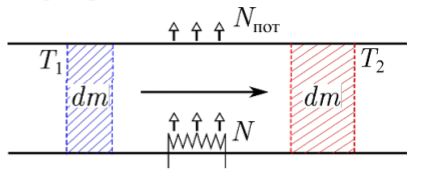
\includegraphics[width=0.6\textwidth]{lab_2_1_1.png}
\label{ris:image}
\end{center}


		 Пусть за некоторое
		 время $dt$ через калориметр прошла
		 малая порция газа массой $dm=q dt$,
		 где $q$ — массовый расход газа в трубе. Если мощность нагрева равна $N$, мощность тепловых потерь на обмен с окружающей средой $N_{\text{пот}}$, то порция получила тепло $\delta Q = (N-N_{\text{пот}})dt$. С другой стороны, по определению теплоёмкости $\delta Q = c dm \Delta T$,  Таким образом $$c_{P} = \frac{N-N_{пот}}{q\Delta T} \; (1).$$
		 
	\section{Экспериментальная установка:}
	
	\begin{center}
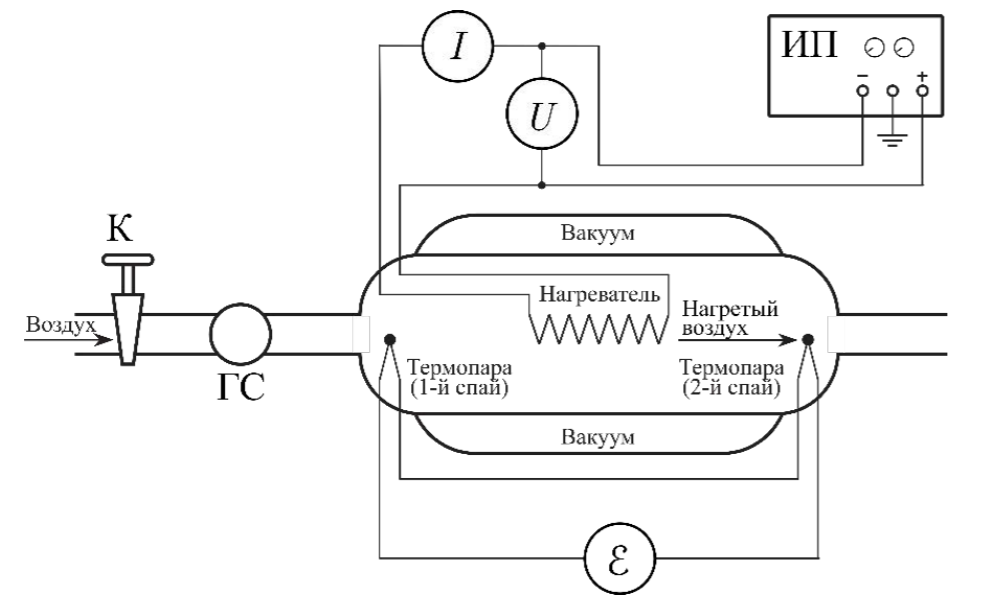
\includegraphics[width=0.6\textwidth]{lab_2_1_1_ust.png}
\label{ris:image}
\end{center}
	
		Мощность нагрева равна
		$N= UI \; $
		
		
		Массовый расход может быть найден как $q = \rho_{0} \frac{\Delta V}{\Delta t} \;$
		
		Мощность потерь тепла $N_{пот}$ прямо пропорциональна разности температур: $ N_{пот} = \alpha \Delta T \; $. При этом условии соотношение (1) принимает вид $$N = (c_{P}q +\alpha)\Delta T \;(2)$$
		Следовательно, при фиксированном расходе воздуха  подводимая мощность и разность температур связаны прямой пропорциональностью($\Delta T(N)$ — линейная функция).

\section{Измерения:}



\end{problem}
\end{document}
